\documentclass[thesis.tex]{subfiles}

\begin{document}
\chapter{Performance testing}
\label{sec:performance}
This chapter is concerned with testing the efficiency of the approach by running large scale tests on the implemented tool. There are two metrics which will be presented: The running time of the algorithm and the correctness of the achieved result. Most of the results are compared against running the same alignment with our own implementation of the PO-MSA algorithm. An explanation on how to find this implementation is given in Appendix \ref{sec:tool}. We chose PO-MSA because of its intuitive nature, the easily deducible relationship between graph complexity and running time and, most importantly, because it is a non-heuristical approach guaranteeing a correct result every time.
\section{Test data}
These tests are meant to reflect usage in what would be an every day situation, and therefore use real genetic data. All of the sequences are FASTA-files from the MHC region fetched from the vg github repo \cite{vg} and the test-set provided by the sequence graphs tool \cite{sequence_graphs}. The exact test sets are chosen to provide a variety of sequence lengths. In order to cover lengths where we found no sequences we created artificial sequences by cutting out suitable regions from longer sequences. All the sequences which are used can be found in the data-folder of the github repo of the tool.\\
\par\noindent
Specifically, there are 8 main data-sets involved in the testing process:
\begin{itemize}
  \item \textbf{mhc1.fa} A 700 bp long sequence from the MHC region (not specified more precisely where). Fetched from the docker repo of the sg project
  \item \textbf{primary.fasta} A 3345 bp long sequence from the HLA-A gene in the MHC region from the primary assembly of GRCh38. Originates from the vg github.
  \item \textbf{20k.fasta, 35k.fasta, 100k.fasta, 150k.fasta, 500k.fasta} Five subsequences of an alternate assembly of the MHC region of respectively 21.070bp, 35.770bp, 101.570bp, 144.480bp and 448.490bp. The alternate assembly originates from the NCBI database\cite{ncbi} with id NT\_167244.1.
  \item \textbf{mhc\_full.fa} The previously mentioned full MHC assembly of 4.622.290bp.
\end{itemize}
Additionally, some of the tests use more specific data to test specific properties. This data will be presented before it is used.\\
\par\noindent
In order to do alignments we need reads aswell as the data used in building the reference structure. These reads are generated by the read generator which is also described in Appendix \ref{sec:tool}. The reads are generated by subtracting a sequence of a given length from the reference graph. In some cases we introduce noise to the reads proportional to a noise probability $p$. The noise is evenly divided among SNPs, insertions and deletions and is uniformly distributed over the entire length of the read. This is a model which is not meant to reflect sequencing errors\footnote{Described in section \ref{sec:sequencing}}, a simplification towards the most general version of the alignment problem.\\
\par\noindent
In detail, the generation of a read $r$ from a graph $G$ happens as follows: 
\begin{enumerate}
  \item Choose a random vertex $v \in V\setminus\{s_G, t_G\}$ such that the smallest distance from $v$ to $t_g$ is larger than the chosen read size $|r|$
  \item For $|r|$ steps:
  \begin{enumerate}
    \item Append $b(v_x)$ to the read $r$
    \item Choose a random neighbouring vertex $v_y \in n_o(v_x)$ as the new $v_x$
  \end{enumerate}
  \item When a read $r$ has been generated, for $r_i \in r$
  \begin{enumerate}
    \item Choose a random floating point value $0<=v<=1$
    \begin{itemize}
      \item If $v<(p/3)$ delete $r_i$
      \item Else if $v<(2p/3)$ insert a random base $b \in \{A, C, G, T\}$ before $r_i$
      \item Else if $v<p$ substitue $r_i$ with a random base $b \in \{A, C, G, T\}\setminus\{r_i\}$
    \end{itemize}
  \end{enumerate}
  \item Output $r$
\end{enumerate}
In order to provide reproducability the randomness in the reads are generated from a seed.\\
\section{Validation}
\label{sec:performance_validation}
When an alignment is produced for a read we classify it as either as correct or not correct. Intuitively one could imagine correctness is determined by whether the generated read aligns back to the path it was generated from. However, when noise is introduced an interesting phenomenon can occur: The modified read can become more similar to another path in the graph than its origin. This can also occur whenever there exists actual equal paths in the graph, typically in the case of repeats. In order to stick with mathemathical properties, our definition of optimality holds no relation to the origin of a read but is purely defined as the path which produces the highest possible alignment score. As PO-MSA is an exhaustive search we define optimally aligned as alignments which produce the same alignment score as the highest score found by PO-MSA. Consequently, as only the scores are compared, even when the approach produces a different alignment than PO-MSA, this is classified as optimal behaviour. Correctness is only discussed in the later stages of the chapter. When we do not add noise to the reads we are able to devises cases where the approach always provide correct results. In all tests where accuracy is omitted this is because the approach had a 100\% success rate.
\par\noindent
\section{Time capturing mechanisms}
For both the "Fuzzy context-based search" and the PO-MSA algorithm the time capturing mechanisms are built into the tool, using the Java System object. This allows us to wrap the time capturing of each individual constituent as close to the functional parts as possible in order to avoid unecessary overhead. When comparing tools the time was taken from the tool was started until the tool ended. Doing it this way has several disadvantages, which are discussed in Section \ref{sec:comparison_tools}. The time unit used throughout the chapter is milliseconds.
\section{Building the index}
\label{sec:building_the_index}
The building of the index is the first step of the process realized through the build\_index.sh script. To summarize this step consists of reading the input files, building the graph and generating the suffix trees. The build process was run 50 times on 6 different data sets, the averaged results can be seen in figure \ref{fig:build_index}. The tool was not able to build an index for the largest input file with ~4.5Mb because of insufficient memory\footnote{Run with 4Gb through the Java parameters -Xmx and -Xms}. Figure \ref{fig:index_constituents} shows the run time broken down into individual constituents.\\

\begin{figure}[!ht]
    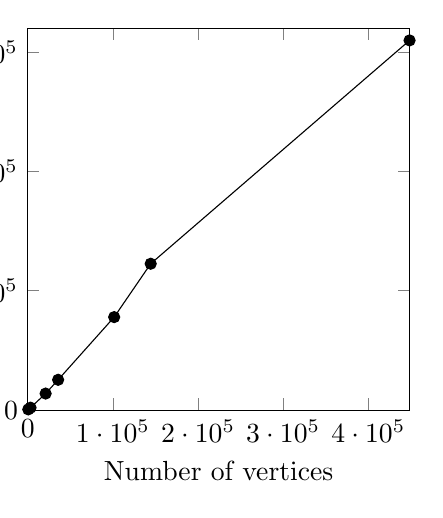
\begin{tikzpicture}[trim axis left, trim axis left]
      \begin{axis}[scale only axis,height=0.4\textwidth,width=0.4\textwidth,xmin=0,ymin=0,xmax=448490,ymax=320000,scaled ticks=false, xlabel={Number of vertices}, ylabel={Milliseconds}, max space between ticks=50pt, ylabel near ticks]
        \addplot[color=black,mark=*] coordinates {
          (700,597)
          (3345,2050)
          (21070,13858)
          (35770,25401)
          (101570,77928)
          (144480,122654)
          (448490,309791)
        };
      \end{axis}
    \end{tikzpicture}
    \caption{Runtime for the build index procedure as a function of the number of vertices}
    \label{fig:build_index}
\end{figure}
\par\noindent
\begin{figure}[!t]
  \begin{subfigure}[t]{0.4\textwidth}
    \begin{tikzpicture}[trim axis left]
      \begin{axis}[scale only axis,height=\textwidth,width=\textwidth,xmin=0,ymin=0,xmax=448490,ymax=320000,scaled ticks=false]
        \addplot coordinates {
          (700,9)
          (3345,51)
          (21070,623)
          (35770,1031)
          (101570,5487)
          (144480,11328)
          (448490,124724)
        };
      \end{axis}
    \end{tikzpicture}
    \subcaption{Time used reading input files and building the graph}
  \end{subfigure}
  \hfill
  \begin{subfigure}[t]{0.4\textwidth}
    \begin{tikzpicture}[trim axis left]
      \begin{axis}[scale only axis,height=\textwidth,width=\textwidth,xmin=0,ymin=0,xmax=448490,ymax=320000,scaled ticks=false]
        \addplot[color=green,mark=*] coordinates {
          (701,65)
          (3345,138)
          (21070,269)
          (35770,2788)
          (101570,6905)
          (144480,10007)
          (448490,15301)
        };
      \end{axis}
    \end{tikzpicture}
    \subcaption{Time used building the index}
  \end{subfigure}
  \begin{subfigure}[b]{0.4\textwidth}
    \begin{tikzpicture}[trim axis left]
      \begin{axis}[scale only axis,height=\textwidth,width=\textwidth,xmin=0,ymin=0,xmax=448490,ymax=320000,scaled ticks=false]
        \addplot[color=red,mark=*] coordinates {
          (700,522)
          (3345,1860)
          (21070,12960)
          (35770,21581)
          (101570,65535)
          (144480,101317)
          (448490,188685)
        };
      \end{axis}
    \end{tikzpicture}
    \subcaption{Time used writing the index\vspace{\baselineskip}}
  \end{subfigure}
  \hfill
  \begin{subfigure}[b]{0.4\textwidth}
  \begin{tikzpicture}[trim axis left]
    \begin{axis}[scale only axis,height=\textwidth,width=\textwidth,xmin=0,ymin=0,xmax=448490,ymax=320000,scaled ticks=false, legend pos=north west]
      \addplot[color=blue,name path=graph] coordinates {
        (700,9)
        (3345,51)
        (21070,623)
        (35770,1031)
        (101570,5487)
        (144480,11328)
        (448490,124724)
      };
      \addplot[color=green, name path=index] coordinates {
        (700,9 + 65)
        (3345,51 + 138)
        (21070,623 + 269)
        (35770,1031 + 2788)
        (101570,5487 + 6905)
        (144480,11328 + 10007)
        (448490,15301 + 124724)
      };
      \addplot[color=red] coordinates {
        (700,597)
        (3345,2050)
        (21070,13858)
        (35770,25401)
        (101570,77928)
        (144480,122654)
      };
      \addplot[color=black, name path=total,mark=*] coordinates {
        (700,597)
        (3345,2050)
        (21070,13858)
        (35770,25401)
        (101570,77928)
        (144480,122654)
        (448490,309791)
      };
      \addplot[name path=axis] coordinates {
        (0, 0)
        (448490, 0)
      };
      \addplot[red!30] fill between[of=index and total];
      \addplot[green!30] fill between[of=graph and index];
      \addplot[blue!30] fill between[of=graph and axis];
      \addlegendimage{only marks, mark=square}
      \addlegendentry{Build graph}
      \addlegendentry{Build index}
      \addlegendentry{Write index}
      \addlegendentry{Total time}
    \end{axis}
  \end{tikzpicture}
  \subcaption{Total run time as a combination of the individual steps}
  \label{fig:index_constituents_explicit}
  \end{subfigure}
  \caption{Time used by the individual constituents of the build index process}
  \label{fig:index_constituents}
\end{figure}
\clearpage
\section{Alignment}
The alignment tests are run by the align\_sequence.sh script, both with \texttt{-{}-type=fuzzy} and \texttt{-{}-type=po\_msa} parameters. As a remainder to the reader, these are the variables which are in play:
\begin{itemize}
  \item $|G|$ is the size of the graph
  \item $\lambda$ is the allowed error margin
  \item $|s|$ is the length of the input sequence
  \item $b$ is the branching factor of the graph
  \item $p$ is the amount of noise added to the reads
\end{itemize}
As each of the subsequent sections are concerned with the impact of exactly one of these variables, the others are locked to a standard value:
\begin{itemize}
  \item $\mathbf{|G|=35.000}$ \\Representing the mid-range of our test-sets.
  \item $\lambda\mathbf{=0, p=0.0}$ \\We let alignment back to the origin represent the base case in the study.
  \item $\mathbf{|s|=120}$ \\Common read length for the Illumina HiSeq3000/4000 technology.
  \item $\mathbf{b=1}$ \\Calculations can be found in section \ref{sec:runtime_complexity}.
\end{itemize}
\subsection*{Runtime as a function of graph size}
We start by comparing the two alignment algorithms on different graph sizes. Figure \ref{fig:runtime_G_log} shows the average results over 50 runs on a log-log scale. Neither of the algorithms managed to handle the largest dataset of ~4Mb because of insufficient memory. PO-MSA also had memory issues and were unable to produce results for the second largest dataset of ~500kb. A linear scale plot of the 6 datasets which both algorithms managed to handle can be seen in figure \ref{fig:runtime_G_small}
\clearpage
\begin{figure}[!ht]
  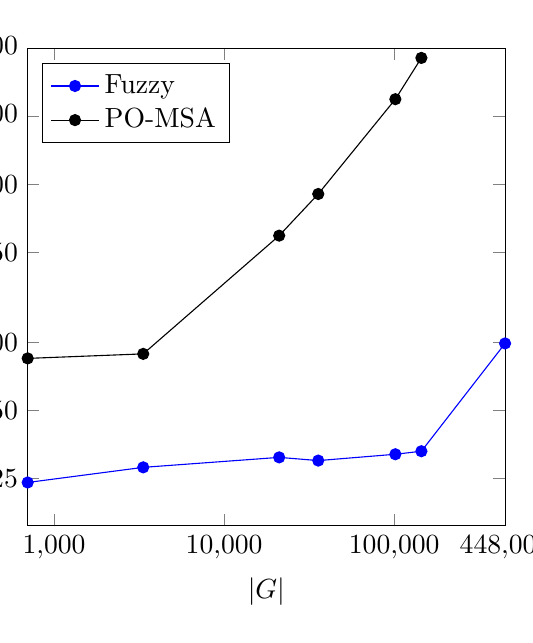
\begin{tikzpicture}[trim axis left, trim axis right]
    \begin{axis}[scale only axis,height=0.5\textwidth,width=0.5\textwidth,xmin=700,ymin=0,xmax=448490,ymax=2000,scaled ticks=false, legend pos=north west, xlabel={$|G|$}, ylabel={Milliseconds}, legend cell align=left, xtick={1000,10000,100000,448490},ylabel near ticks, xmode=log, ymode=log, log ticks with fixed point, ytick={25, 50, 100, 250, 500, 1000, 2000}]
      \addplot[color=blue,mark=*] coordinates {
        (700, 24)
        (3345, 28)
        (21070, 31)
        (35770,  30)
        (101570, 32)
        (144480, 33)
        (448490, 99)
      };
      \addplot[color=black,mark=*] coordinates {
        (700, 85)
        (3345, 89)
        (21070, 297)
        (35770, 454)
        (101570, 1193)
        (144480, 1817)
      };
      \addlegendentry{Fuzzy}
      \addlegendentry{PO-MSA}
    \end{axis}
  \end{tikzpicture}
  \caption{Runtime of the alignment process as a function of $|G|$ on a log-log scale for the 7 smallest datasets}
  \label{fig:runtime_G_log}
\end{figure}
\begin{figure}[!hb]
  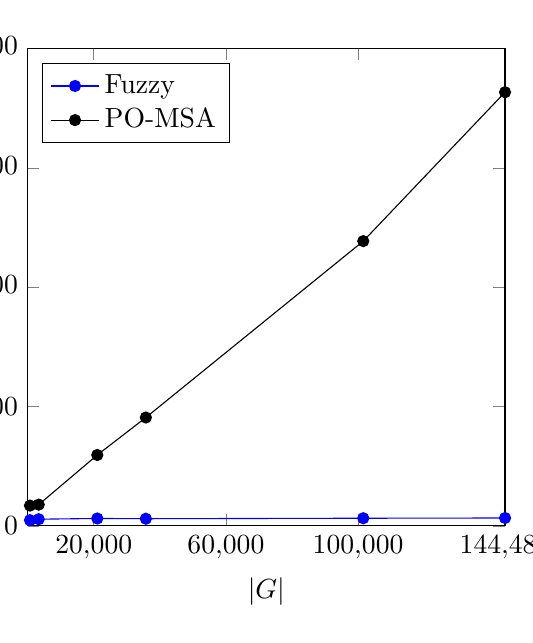
\begin{tikzpicture}[trim axis left, trim axis right]
    \begin{axis}[scale only axis,height=0.5\textwidth,width=0.5\textwidth,xmin=0,ymin=0,xmax=144480,ymax=2000,scaled ticks=false, legend pos=north west, xlabel={$|G|$}, ylabel={Milliseconds}, legend cell align=left,ylabel near ticks,xtick={20000,60000,100000,144480},xticklabel style={/pgf/number format/fixed}]
      \addplot[color=blue,mark=*] coordinates {
        (700, 24)
        (3345, 28)
        (21070, 31)
        (35770,  30)
        (101570, 32)
        (144480, 33)
      };
      \addplot[color=black,mark=*] coordinates {
        (700, 85)
        (3345, 89)
        (21070, 297)
        (35770, 454)
        (101570, 1193)
        (144480, 1817)
      };
      \addlegendentry{Fuzzy}
      \addlegendentry{PO-MSA}
    \end{axis}
  \end{tikzpicture}
  \caption{Runtime of the alignment process as a function of $|G|$ on a linear scale for the 6 smallest datasets}
  \label{fig:runtime_G_small}
\end{figure}
\clearpage
\subsection*{Runtime as a function of error margin}
We vary the error margin by giving the algorithm different $\lambda$-values through the \texttt{-{}-error-margin} parameter. The results from 50 runs at 5 different values are seen in figure \ref{fig:runtime_lambda}. Figure \ref{fig:runtime_lambda_parallell} shows the same set of tests on the larger graph and includes a plot for an equivalent set of tests run with the \texttt{-{}-parallellization=true} parameter.
\begin{figure}[!ht]
  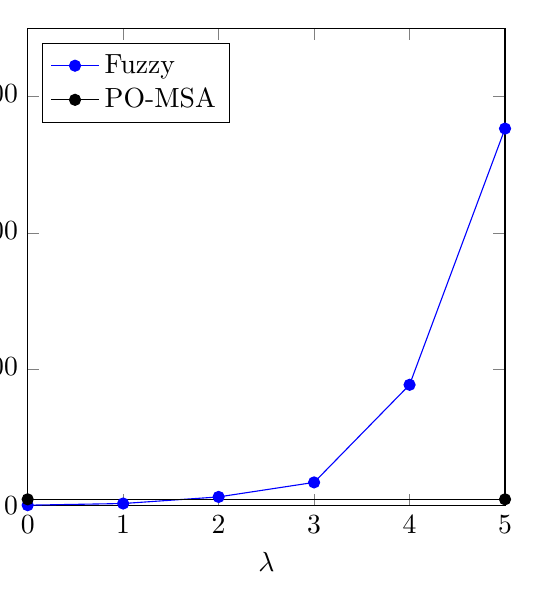
\begin{tikzpicture}[trim axis left, trim axis right]
    \begin{axis}[scale only axis,height=0.5\textwidth,width=0.5\textwidth,xmin=0,ymin=0,xmax=5,ymax=35000,scaled ticks=false, legend pos=north west, xlabel={$\lambda$}, ylabel={Milliseconds},xtick={0,1,2,3,4,5}, legend cell align=left, ylabel near ticks]
      \addplot[color=blue,mark=*] coordinates {
        (0, 29)
        (1, 152)
        (2, 636)
        (3, 1700)
        (4, 8856)
        (5, 27642)
      };
      \addplot[color=black,mark=*] coordinates {
        (0, 460)
        (5, 460)
      };
      \addlegendentry{Fuzzy}
      \addlegendentry{PO-MSA}
    \end{axis}
  \end{tikzpicture}
  \caption{Runtime of the alignment process as a function of $\lambda$}
  \label{fig:runtime_lambda}
\end{figure}
\begin{figure}[!hb]
  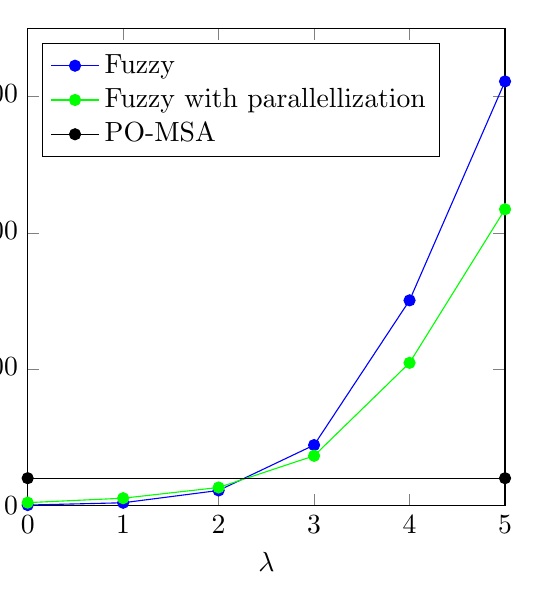
\begin{tikzpicture}[trim axis left, trim axis right]
    \begin{axis}[scale only axis,height=0.5\textwidth,width=0.5\textwidth,xmin=0,ymin=0,xmax=5,ymax=35000,scaled ticks=false, legend pos=north west, xlabel={$\lambda$}, ylabel={Milliseconds},xtick={0,1,2,3,4,5}, legend cell align=left, ylabel near ticks]
      \addplot[color=blue,mark=*] coordinates {
        (0, 39)
        (1, 207)
        (2, 1109)
        (3, 4438)
        (4, 15048)
        (5, 31101)
      };
      \addplot[color=green,mark=*] coordinates {
        (0,217)
        (1,541)
        (2,1327)
        (3,3649)
        (4,10466)
        (5,21725)
      };
      \addplot[color=black,mark=*] coordinates {
        (0, 2008)
        (5, 2008)
      };
      \addlegendentry{Fuzzy}
      \addlegendentry{Fuzzy with parallellization}
      \addlegendentry{PO-MSA}
    \end{axis}
  \end{tikzpicture}
  \caption[Runtime of the alignment process as a function of $\lambda$ with a larger data set]{Runtime of the alignment process as a function of $\lambda$ with $|G|=150.000$ and \texttt{-{}-parallellization=true}}
  \label{fig:runtime_lambda_parallell}
\end{figure}
\clearpage
\subsection*{Runtime as a function of sequence length}
We vary the sequence lengths through changing the lengths produced by the read generator. The read lengths are chosen to reflect a variety of sequencing machines, displaying a diversity in read lengths \cite{sequencing_platforms}\cite{comparison_sequencing_systems}. Both the technologies, the lengths and the runtimes are listed in table \ref{tab:runtimes_s}. The number are visualized in figure \ref{fig:runtime_s}
\begin{table}[!h]
  \begin{tabular}{|l|l|r|r|}
    \hline \textbf{Technology} & \textbf{Read length} & \textbf{PO-MSA time} & \textbf{Fuzzy time} \\ \hline
    HiSeq2000 (min) & 50 & 171 & 19 \\ \hline
    SOLiDv4 & 100 & 294 & 36 \\ \hline
    HiSeq3000/4000 & 120 & 545 & 39 \\ \hline
    Ion PGM & 200 & 676 & 59 \\ \hline
    Sanger 3730xl (min) & 400 & 1117 & 98 \\ \hline
    454 GS FLX & 700 & 1600 & 167 \\ \hline
    Sanger 3730xl (max) & 900 & 2121 & 194 \\ \hline
  \end{tabular}
  \caption{Running times for reads produced by different sequencing technologies for the PO-MSA and fuzzy search algorithm}
  \label{tab:runtimes_s}
\end{table}
\begin{figure}[!hb]
  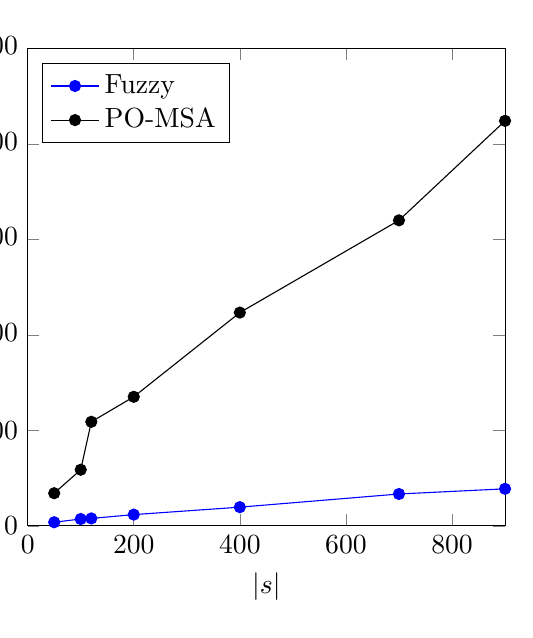
\begin{tikzpicture}[trim axis left, trim axis right]
    \begin{axis}[scale only axis,height=0.5\textwidth,width=0.5\textwidth,xmin=0,ymin=0,xmax=900,ymax=2500,scaled ticks=false, legend pos=north west, xlabel={$|s|$}, ylabel={Milliseconds}, legend cell align=left, ylabel near ticks]
      \addplot[color=blue,mark=*] coordinates {
        (50,19)
        (100,36)
        (120,39)
        (200,59)
        (400,98)
        (700,167)
        (900,194)
      };
      \addplot[color=black,mark=*] coordinates {
        (50,171)
        (100,294)
        (120,545)
        (200,676)
        (400,1117)
        (700,1600)
        (900,2121)
      };
      \addlegendentry{Fuzzy}
      \addlegendentry{PO-MSA}
    \end{axis}
  \end{tikzpicture}
  \caption{Runtime of the alignment process as a function of $|s|$}
  \label{fig:runtime_s}
\end{figure}
\clearpage
\subsection*{Runtime as a function of graph complexity}
\label{sec:runtime_complexity}
We let the branching probability $b$ denote the complexity of our graph. This is a factor computed as a function of the relationship between the number of vertices and the number of edges. We created variation through generating a set of VCF files\footnote{The variant file format mentioned in section \ref{sec:sequencing} } with the read generator to provide a variety of values. The results of running alignments against each of the indexes can be seen in figure \ref{fig:runtime_b}.\\
\par\noindent
If we use the numbers from the 1000 genomes project from 2010 \cite{a_map_of_human_genome_variation_from_population_scale_sequencing} we can approximate a branching factor $b\approx1.0066$ for a population of 179 individuals \footnote{14.894.361 SNPs + 3.019.909 indels +  21.075 structural variations / 2.420.000.000bp}. At the completion of the project, \textasciitilde88 million variants had been found in a population of 2504, indicating the factor $b\approx1.029$ \cite{1000_genomes_global_ref}. Both of these data points are visualized in the plot.
\begin{figure}[!hb]
  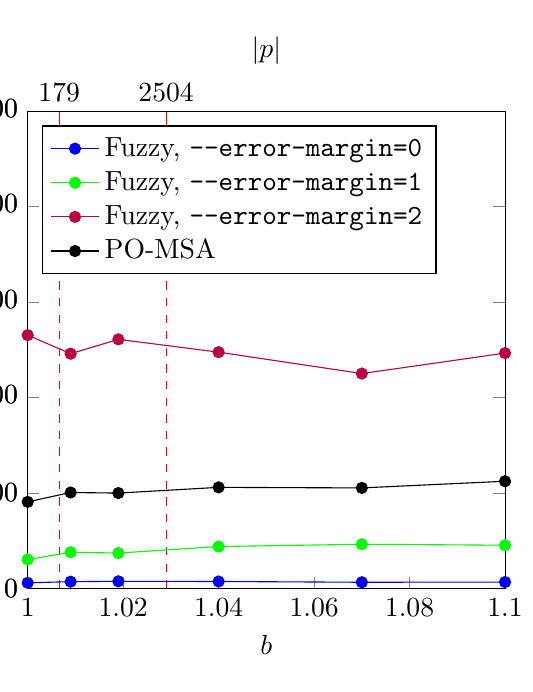
\begin{tikzpicture}[trim axis left, trim axis right]

\begin{axis}[scale only axis,height=0.5\textwidth,width=0.5\textwidth,xmin=1,ymin=0,ymax=2500,xmax=1.1,scaled ticks=false,xlabel={$|p|$}, axis x line*=top, xlabel near ticks,xtick={1.0066, 1.029},xticklabels={179, 2504}]
        \addplot[color=red, style=dashed] coordinates {
          (1.0066,0)
          (1.0066,1640)
      };
   \addplot[color=red] coordinates {
          (1.0066,2500)
          (1.0066,2420)
      };
        \addplot[color=red, style=dashed] coordinates {
          (1.029,0)
          (1.029,1640)
      };
   \addplot[color=red] coordinates {
          (1.029,2500)
          (1.029,2420)
      };
    \end{axis}
    \begin{axis}[scale only axis,height=0.5\textwidth,width=0.5\textwidth,xmin=1,ymin=0,ymax=2500,xmax=1.1,scaled ticks=false, legend pos=north west, xlabel={$b$}, ylabel={Milliseconds}, legend cell align=left, ylabel near ticks, xtick pos=left]
      \addplot[color=blue,mark=*] coordinates {
        (1,30)
        (1.009,36)
        (1.019,38)
        (1.04,37)
        (1.07,33)
        (1.1,34)
      };
      \addplot[color=green,mark=*] coordinates {
        (1,152)
        (1.009,190)
        (1.019,186)
        (1.04,220)
        (1.07,232)
        (1.1,227)
      };
      \addplot[color=purple,mark=*] coordinates {
        (1,1327)
        (1.009,1230)
        (1.019,1305)
        (1.04,1238)
        (1.07,1126)
        (1.1,1233)
      };
      \addplot[color=black,mark=*] coordinates {
        (1,454)
        (1.009,503)
        (1.019,500)
        (1.04,530)
        (1.07,527)
        (1.1,562)
      };
      \addlegendentry{Fuzzy, \texttt{-{}-error-margin=0}}
      \addlegendentry{Fuzzy, \texttt{-{}-error-margin=1}}
      \addlegendentry{Fuzzy, \texttt{-{}-error-margin=2}}
      \addlegendentry{PO-MSA}
    \end{axis}
  \end{tikzpicture}
  \caption{Runtime of the alignment process as a function of $b$. Datapoints depicting population sizes from earlier studies are shown as red vertical lines}
  \label{fig:runtime_b}
\end{figure}
\clearpage
\subsection*{Accuracy as a function of noise}
In the previous tests we have guaranteed correct results through the tuning of input parameters. We will now introduce a level of uncertainty through introducing randomness to our reads through the noise parameter $p$. To some degree this is a futile exercise: We will get correct results when the number of modifications is lower than $\lambda$ and empty alignments in the remaining cases, mirroring the distribution of the underlying randomness. This is however interesting as a depiction of a real life situation where the noise is to some degree uncertain. The percentage of correctly aligned reads over a total of 3600 runs with a variety of settings is seen in \ref{fig:correctness_both}. In this set of tests we also include the results from the heuristical algorithm, shown in \ref{fig:correctness_both_heur}.
\begin{figure}[!hb]
\captionsetup[subfigure]{justification=centering}
  \begin{subfigure}[t]{0.49\textwidth}
  \begin{center}
    \begin{tikzpicture}[every node/.style={anchor=base,text depth=.5ex,text height=1.55em,text width=1.55em},align=center,text centered, trim axis left, trim axis right]
      \matrix(A) [nodes={rectangle}] {
        \node {5}; & \HeatmapNode{100} & \HeatmapNode{100} & \HeatmapNode{99} & \HeatmapNode{96} & \HeatmapNode{83} & \HeatmapNode{80}\\
        \node {4}; & \HeatmapNode{100} & \HeatmapNode{99} & \HeatmapNode{96} & \HeatmapNode{83} & \HeatmapNode{73} & \HeatmapNode{40}\\
        \node {3}; & \HeatmapNode{100} & \HeatmapNode{97} & \HeatmapNode{86} & \HeatmapNode{66} & \HeatmapNode{36} & \HeatmapNode{20}\\
        \node {2}; & \HeatmapNode{100} & \HeatmapNode{92} & \HeatmapNode{68} & \HeatmapNode{30} & \HeatmapNode{12} & \HeatmapNode{9}\\
        \node {1}; & \HeatmapNode{100} & \HeatmapNode{74} & \HeatmapNode{43} & \HeatmapNode{11} & \HeatmapNode{5} & \HeatmapNode{5}\\
        \node {0}; & \HeatmapNode{100} & \HeatmapNode{38} & \HeatmapNode{13} & \HeatmapNode{3} & \HeatmapNode{2} & \HeatmapNode{0}\\
        \node {};  & \node{0}; & \node{0.01}; & \node{0.02}; & \node{0.03}; & \node{0.04}; & \node{0.05}; \\
      };
      \node[draw=none] at (0.5, -0.75) {$p$};
      \node[draw=none] at (-3, 3.25) {$\lambda$};
    \end{tikzpicture}
  \subcaption{Results from the tool with default \\settings}
    \label{fig:correctness_both}
\end{center}
  \hfill
  \end{subfigure}
    \begin{subfigure}[t]{0.49\textwidth}
  \begin{center}
    \begin{tikzpicture}[every node/.style={anchor=base,text depth=.5ex,text height=1.55em,text width=1.55em},align=center,text centered, trim axis left, trim axis right]
      \matrix(A) [nodes={rectangle}] {
        \node {5}; & \HeatmapNode{100} & \HeatmapNode{100} & \HeatmapNode{100} & \HeatmapNode{100} & \HeatmapNode{100} & \HeatmapNode{100}\\
        \node {4}; & \HeatmapNode{100} & \HeatmapNode{100} & \HeatmapNode{100} & \HeatmapNode{100} & \HeatmapNode{97} & \HeatmapNode{98}\\
        \node {3}; & \HeatmapNode{100} & \HeatmapNode{99} & \HeatmapNode{99} & \HeatmapNode{97} & \HeatmapNode{83} & \HeatmapNode{86}\\
        \node {2}; & \HeatmapNode{100} & \HeatmapNode{98} & \HeatmapNode{96} & \HeatmapNode{88} & \HeatmapNode{62} & \HeatmapNode{58}\\
        \node {1}; & \HeatmapNode{100} & \HeatmapNode{92} & \HeatmapNode{79} & \HeatmapNode{54} & \HeatmapNode{38} & \HeatmapNode{26}\\
        \node {0}; & \HeatmapNode{100} & \HeatmapNode{53} & \HeatmapNode{21} & \HeatmapNode{6} & \HeatmapNode{4} & \HeatmapNode{1}\\
        \node {};  & \node{0}; & \node{0.01}; & \node{0.02}; & \node{0.03}; & \node{0.04}; & \node{0.05}; \\
      };
      \node[draw=none] at (0.5, -0.75) {};
    \end{tikzpicture}
  \subcaption{Results from the tool run with \\the parameter\texttt{-{}-heuristical=true}}
  \label{fig:correctness_both_heur}
  \end{center}
  \end{subfigure}
  \caption[Percentage of correctly mapped reads]{Percentage of correctly aligned reads as a function of both $p$ and $\lambda$. Each cell in the heatmap represents one setting}
  \label{fig:correctness}
\end{figure}
\clearpage
\section{Comparison with the sequence graphs tool}
In this section we will compare the GraphGenome tool with the sequence graphs tool (sg) created by Novak et al. as an implementation of the algorithm presented in the article "Canonical, Stable, General Mapping using Context Schemes". On the github page \cite{sg_git} the creators state:
\begin{displayquote}
``Indeed, the tool to align sequences to the index is currently unfinished.''
\end{displayquote}
Additionally, we did not manage to run the tool on larger datasets. For these reasons the sg tool has not been used as a benchmark for the remaining tests, but only been granted this section.\\
\par\noindent
 The two tools were compared in building the index and doing an alignment, the results can be seen in respectively figure \ref{fig:comparison_build} and \ref{fig:comparison_align}. Because of the limitations with regards to graph size, we have introduced several smaller sample fasta-files found in their test-folder as input data. We have divided the execution time of the GraphGenome tool into ``functional'' time and file I/O to indicate the level of overhead which is expected when doing comparisons of execution times for complete tools.
\label{sec:comparison_tools}
\begin{figure}[!hb]
  \begin{tikzpicture}[trim axis left, trim axis right]
    \begin{axis}[scale only axis,height=0.5\textwidth,width=0.5\textwidth,xmin=140,ymin=0,xmax=7000,ymax=2750,scaled ticks=false,xtick={140,1000,3000,5000,7000}, legend pos=north west, xlabel={$|G|$}, ylabel={Milliseconds}]
      \addplot[color=blue,mark=*, name path=index] coordinates {
      	(140,4+11)
        (700,8+22)
        (2000,20+57)
        (3345,29+61)
        (7000,64+81)
      };
      \addplot[color=red, name path=total,mark=*] coordinates {
      	(140,515)
        (700,559)
        (2000,1128)
        (3345,1408)
        (7000,2563)
      };
      \addplot[color=black, name path=vg,mark=*] coordinates {
      	(140,1087)
      	(700,1084)
      	(2000,1091)
        (3345,1093)
        (7000,1125)
      };
      \addplot[name path=axis] coordinates {
        (0, 0)
        (7000, 0)
      };
      \addplot[red!30] fill between[of=index and total];
      \addplot[blue!30] fill between[of=axis and index];
      \addlegendentry{Fuzzy algorithm time}
      \addlegendentry{Fuzzy tool time}
      \addlegendentry{Sequence graphs tool time}
    \end{axis}
  \end{tikzpicture}
  \caption[Time spent building the index by the two tools]{Time spent building the index by the two tools. The red line indicates the total time spent by the GraphGenome tool. The red section indicates file I/O, the blue section indicates time spent by the fuzzy search algorithm}
  \label{fig:comparison_build}
\end{figure}
\clearpage\noindent
\begin{figure}[H]
  \begin{tikzpicture}[trim axis left, trim axis right]
    \begin{axis}[scale only axis,height=0.5\textwidth,width=0.5\textwidth,xmin=140,ymin=0,xmax=7000,ymax=2500,scaled ticks=false,xtick={140,1000,3000,5000,7000}, legend pos=north west, xlabel={$|G|$}, ylabel={Milliseconds}]
      \addplot[color=blue,mark=*, name path=index] coordinates {
      	(140,28)
        (700,28)
        (2000,29)
        (3345,28)
        (7000,31)
      };
      \addplot[color=red, name path=total,mark=*] coordinates {
      	(140,364)
        (700,539)
        (2000,948)
        (3345,1272)
        (7000,2241)
      };
      \addplot[color=black, name path=vg,mark=*] coordinates {
      	(104,1015)
      	(700,1018)
      	(2000,1022)
        (3345,1024)
        (7000,1032)
      };
      \addplot[name path=axis] coordinates {
        (0, 0)
        (7000, 0)
      };
      \addplot[red!30] fill between[of=index and total];
      \addplot[blue!30] fill between[of=axis and index];
      \addlegendentry{Fuzzy algorithm time}
      \addlegendentry{Fuzzy tool time}
      \addlegendentry{Sequence graphs tool time}
    \end{axis}
  \end{tikzpicture}
  \caption{Runtimes of alignment by the two tools}
  \label{fig:comparison_align}
\end{figure}
\noindent
The sg tool has a \texttt{-{}-mismatch} parameter which works similarly to our \texttt{-{}-error-margin} parameter by putting a bound on the allowed number of mismatches. The accuracy of the two tools over varying amounts of noise with a set mismatch and error-margin parameter can be seen in figure \ref{fig:comparison_correctness}.
\begin{figure}[H]
  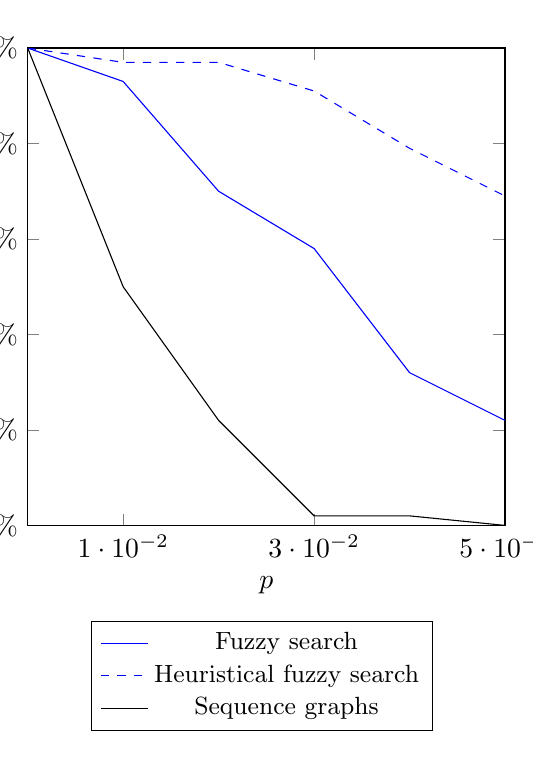
\begin{tikzpicture}[trim axis left,trim axis right]
    \begin{axis}[scale only axis,height=0.5\textwidth,width=0.5\textwidth,xmin=0,ymin=0,xmax=0.05,ymax=100,scaled ticks=false,xtick={0.01,0.03,0.05}, ytick={0,20,40,60,80,100}, yticklabels={0\%,20\%,40\%,60\%,80\%,100\%},ylabel={Percentage of correctly mapped reads}, xlabel={$p$}, legend style={font=\small, at={(0.85,-0.2)}}]
      \addplot[color=blue] coordinates {
        (0, 100-0)
        (0.01,100-7)
        (0.02,100-30)
        (0.03,100-42)
        (0.04,100-68)
        (0.05,100-78)
      };
      \addplot[color=blue, style=dashed] coordinates {
        (0, 100)
        (0.01, 97)
        (0.02, 97)
        (0.03, 91)
        (0.04, 79)
        (0.05, 69)
      };
      \addplot[color=black] coordinates {
        (0, 100-0)
        (0.01,100-50)
        (0.02,100-78)
        (0.03,100-98)
        (0.04,100-98)
        (0.05,100-100)
      };
      \addlegendentry{Fuzzy search}
      \addlegendentry{Heuristical fuzzy search}
      \addlegendentry{Sequence graphs}
    \end{axis}
  \end{tikzpicture}
  \caption[Accuracy of the two tools]{Accuracy of the two tools with $\lambda=2$. The dashed line indicates the accuracy of the GraphGenome tool with the parameter \texttt{-{}-heuristical=true}}
  \label{fig:comparison_correctness}
\end{figure}
\end{document}